\graphicspath{{2Layer_QG/code/plot_snap/figs/}}
\renewcommand{\Bu}{\text{Bu}}

% \section{The full model nondimensionalized}
% We start with the 2 layer QG model with mean flow, $\beta$, and topography \parencite[(5.85-86)]{Vallis_17} (in the notation of \cite{Vallis_96a}):
% \begin{align}
%     &\frac{\pe q_1}{\pe t}+J(\psi_1,q_1)+U_1\frac{\pe q_1}{\pe x}+\left(\{\xi_1^{-2}\}\beta+\{\Bu_1^{-1}\}\frac{f_0^2(U_1-\{U_r\}U_2)}{g'H_1}\right)\frac{\pe\psi_1}{\pe x} = 0;\label{eq:2lay_eq1}\\
%     \{A\}&\frac{\pe q_2}{\pe t}+J(\psi_2,q_2)+U_2\frac{\pe q_2}{\pe x}+\left(\{\xi_2^{-2}\}\beta+\{\Bu_2^{-1}\}\frac{f_0^2(U_2-\{U_r^{-1}\}U_1)}{g'H_2}\right)\frac{\pe\psi_2}{\pe x} = 0.\label{eq:2lay_eq2}
% \end{align}
% where
% \begin{align}
%     q_1 &= \nabla^2\psi_1 + \{\Bu_1^{-1}\}\frac{f_0^2}{g'H_1}(\{U_r\}\psi_2-\psi_1);\label{eq:2lay_pv1}\\
%     q_2 &= \nabla^2\psi_2 + \{\Bu_2^{-1}\}\frac{f_0^2}{g'H_2}(\{U_r^{-1}\}\psi_1-\psi_2)+\left\{\frac{\alpha}{\text{Ro}_2}\right\}\frac{f_0}{H_2}\eta.\label{eq:2lay_pv2}
% \end{align}
% We have nondimensionalized time to be the advective timescale of the first layer:
% \begin{align}
%     T = \frac{L_1}{U_1}.
% \end{align}
% Then we nondimensionalized \eqref{eq:2lay_eq1} and \eqref{eq:2lay_pv1} with length $L_1$ and \eqref{eq:2lay_eq2} and \eqref{eq:2lay_pv2} with length $L_2$. We have introduced the nondimensional number $\xi$ which is the ratio between the Rhine scale and the lengthscale of each layer \parencite{HeldLarichev_96}
% \begin{align}
%     \xi_i^{-2} = \frac{\beta L_i^2}{|U_i|}
% \end{align}
% and $\alpha$ which is the ratio of the typical topographic height versus the second layer's height
% \begin{align}
%     \alpha = \frac{\eta}{H_2}.
% \end{align}
% If the height and mean flow of the two layers are not equal, we have two parameters for their ratio
% \begin{align}
%     U_r = \frac{|U_2|}{|U_1|}, \qdt{and} A = \frac{|U_1|L_2}{|U_2|L_1}
% \end{align}
% We also have the more familiar quantities
% \begin{align}
%     L_{i,d} = \frac{\sqrt{g'H_i}}{f_0} \qdt{,} \text{Ro}_2 = \frac{|U_2|}{f_0L_2} \qdt{and} \text{Bu}_i = \frac{L_{i,d}^2}{L_i^2}.
% \end{align}

\section{The symmetric, flat bottom model}
\subsection{The nondimensional equations}
The 2 layer model simplifies drastically when we make the upper/lower layer symmetry assumption \parencite{LarichevHeld_95}. We take $H_1=H_2 = H/2$ and $U_1=-U_2=U$. Then the equation becomes
\begin{align}
    &\frac{\pe q_1}{\pe t}+J(\psi_1,q_1)+U\frac{\pe q_1}{\pe x}+\left(\{\xi^{-2}\}\beta+\{8\Bu^{-1}\}\frac{4f_0^2U}{g'H}\right)\frac{\pe\psi_1}{\pe x} = 0,\label{eq:2lay_sym_eq1}\\
    &\frac{\pe q_2}{\pe t}+J(\psi_2,q_2)-U\frac{\pe q_2}{\pe x}+\left(\{\xi^{-2}\}\beta-\{8\Bu^{-1}\}\frac{4f_0^2U}{g'H}\right)\frac{\pe\psi_2}{\pe x} = 0;\label{eq:2lay_sym_eq2}
\end{align}
where
\begin{align}
    q_1 &= \nabla^2\psi_1 + \{4\Bu^{-1}\}\frac{2f_0^2}{g'H}(\psi_2-\psi_1),\label{eq:2lay_sym_pv1}\\
    q_2 &= \nabla^2\psi_2 + \{4\Bu^{-1}\}\frac{2f_0^2}{g'H}(\psi_1-\psi_2)+\left\{\frac{\alpha}{\text{Ro}}\right\}\frac{2f_0}{H}\eta.\label{eq:2lay_sym_pv2}
\end{align}
We have 
\begin{align}
    \xi^{-2} = \frac{\beta L^2}{U} \qdt{,} \text{Bu} = \frac{2g'H}{f_0^2L^2} = \frac{L_{d}^2}{L^2} \qdt{and} \alpha = \frac{2\eta}{H}.
\end{align}
Note that this implies (cf. \cite[(9.103)]{Vallis_17})
\begin{align}
    L_d = \frac{2\sqrt{g'H/2}}{f_0} \qdt{with} k_d^2 = \frac{4f_0^2}{g'H} = \frac{8}{L_d^2}.
\end{align}
This is an ok definition when we connect to the continuously stratified case by using (cf. \cite[(5.138)]{Vallis_17})
\begin{align}
    L_d = \frac{NH}{f} \qdt{with} N^2 = \frac{g'}{H/2}.
\end{align}
$\xi$ and $\Bu$ are not independent since their only freedom is in picking $L$. In our simulation, we pick $L=L_d$ such that $\text{Bu}=1$. 
We further simplify by setting flat topography ($\alpha=0$). The only free parameter is $\xi$
\begin{align}
    \xi^{-2}= \frac{\beta L^2}{U} = \frac{\beta L_d^2}{U}
\end{align}
It is the two-layer version of the `Charney–Green number’. 

Finally, we simulate using a $|k|^8$ hyper-diffusivity on $q_i$ for small scale dissipation and an Ekman damping only in the bottom layer for damping the inverse cascade.

\subsection{Linear stability analysis}
We take only the linear terms of the above model, and dispense of all unnecessary parameters:
\begin{align}
    &\frac{\pe q_1}{\pe t}+\frac{\pe q_1}{\pe x}+\left(\xi^{-2}+8\Bu^{-1}\right)\frac{\pe\psi_1}{\pe x} = 0,\label{eq:2lay_sym_eq1_lin}\\
    &\frac{\pe q_2}{\pe t}-\frac{\pe q_2}{\pe x}+\left(\xi^{-2}-8\Bu^{-1}\right)\frac{\pe\psi_2}{\pe x} = 0;\label{eq:2lay_sym_eq2_lin}
\end{align}
where
\begin{align}
    q_1 &= \nabla^2\psi_1 + 4\Bu^{-1}(\psi_2-\psi_1),\label{eq:2lay_sym_pv1_lin}\\
    q_2 &= \nabla^2\psi_2 + 4\Bu^{-1}(\psi_1-\psi_2).\label{eq:2lay_sym_pv2_lin}
\end{align}

This system if isomorphic to \cite[(9.107)]{Vallis_17}. Therefore we can copy down the answer:
\begin{align}
    c &= -\frac{\xi^{-2}}{K^2+8\Bu^{-1}}\left\{ 1+\frac{8\Bu^{-1}}{2K^2}\pm\frac{8\Bu^{-1}}{2K^2}\left[1+4\frac{K^4(K^4-8^2\Bu^{-2})}{8^2\xi^{-4}\Bu^{-2}}\right]^{1/2} \right\}.
\end{align}
We have recovered \cite[(9.114)]{Vallis_17} with $\hat{k}_d^2 = 8$ and (cf. \cite[(9.115)]{Vallis_17})
\begin{align}
    \xi^{-2} = \hat{k}_\beta^2 = \frac{\beta L_d^2}{U}.
\end{align}

Now we can use the eigenvalue-problem module of Dedalus is solve the same problem numerically. Figure \ref{fig:2Lay_linstab} shows the growth rate. This is a reproduction of \cite[Fig. 9.14]{Vallis_17}.
\begin{figure}
    \centering
    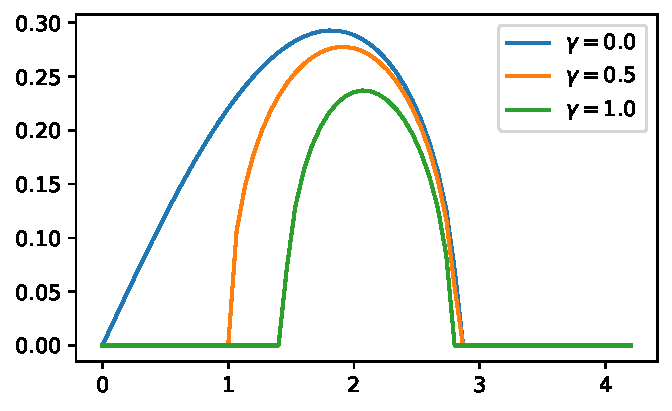
\includegraphics{2Lay_linstab}
    \caption{}
    \label{fig:2Lay_linstab}
\end{figure}


\subsection{Simulation of jets formation}
We pick $\xi = 0.4$ for a large $\zeta$ effect while still having a baroclinically unstable background. At early times, baroclinic instability appears with its distinct pattern. In Figure \ref{fig:2Layjets_q1_t6d50} we also plot a sin wave with $2.26$ wavenumber, the fastest growing mode for $\xi = 0.4$. We see that the instability pattern matches the theory. At later times, the flow develops into jets. Figure \ref{fig:2Layjets_q1_t150d00} shows clear PV staircases with homogenized regions in between. Figure \ref{fig:2Layjets_q1zonalmean_t150d00} plots the zonally averaged perturbation PV $q_1$ against a sin wave of wavenumber $1/2\xi$. We see that matches well the distance between jets. Note that
\begin{align}
    \frac{1}{2\xi} = \frac{1}{2}\hat{k}_\beta = \sqrt{\gamma}
\end{align}
where $\gamma$ is defined in \cite[(9.115)]{Vallis_17}. 

\begin{figure}
    \centering
    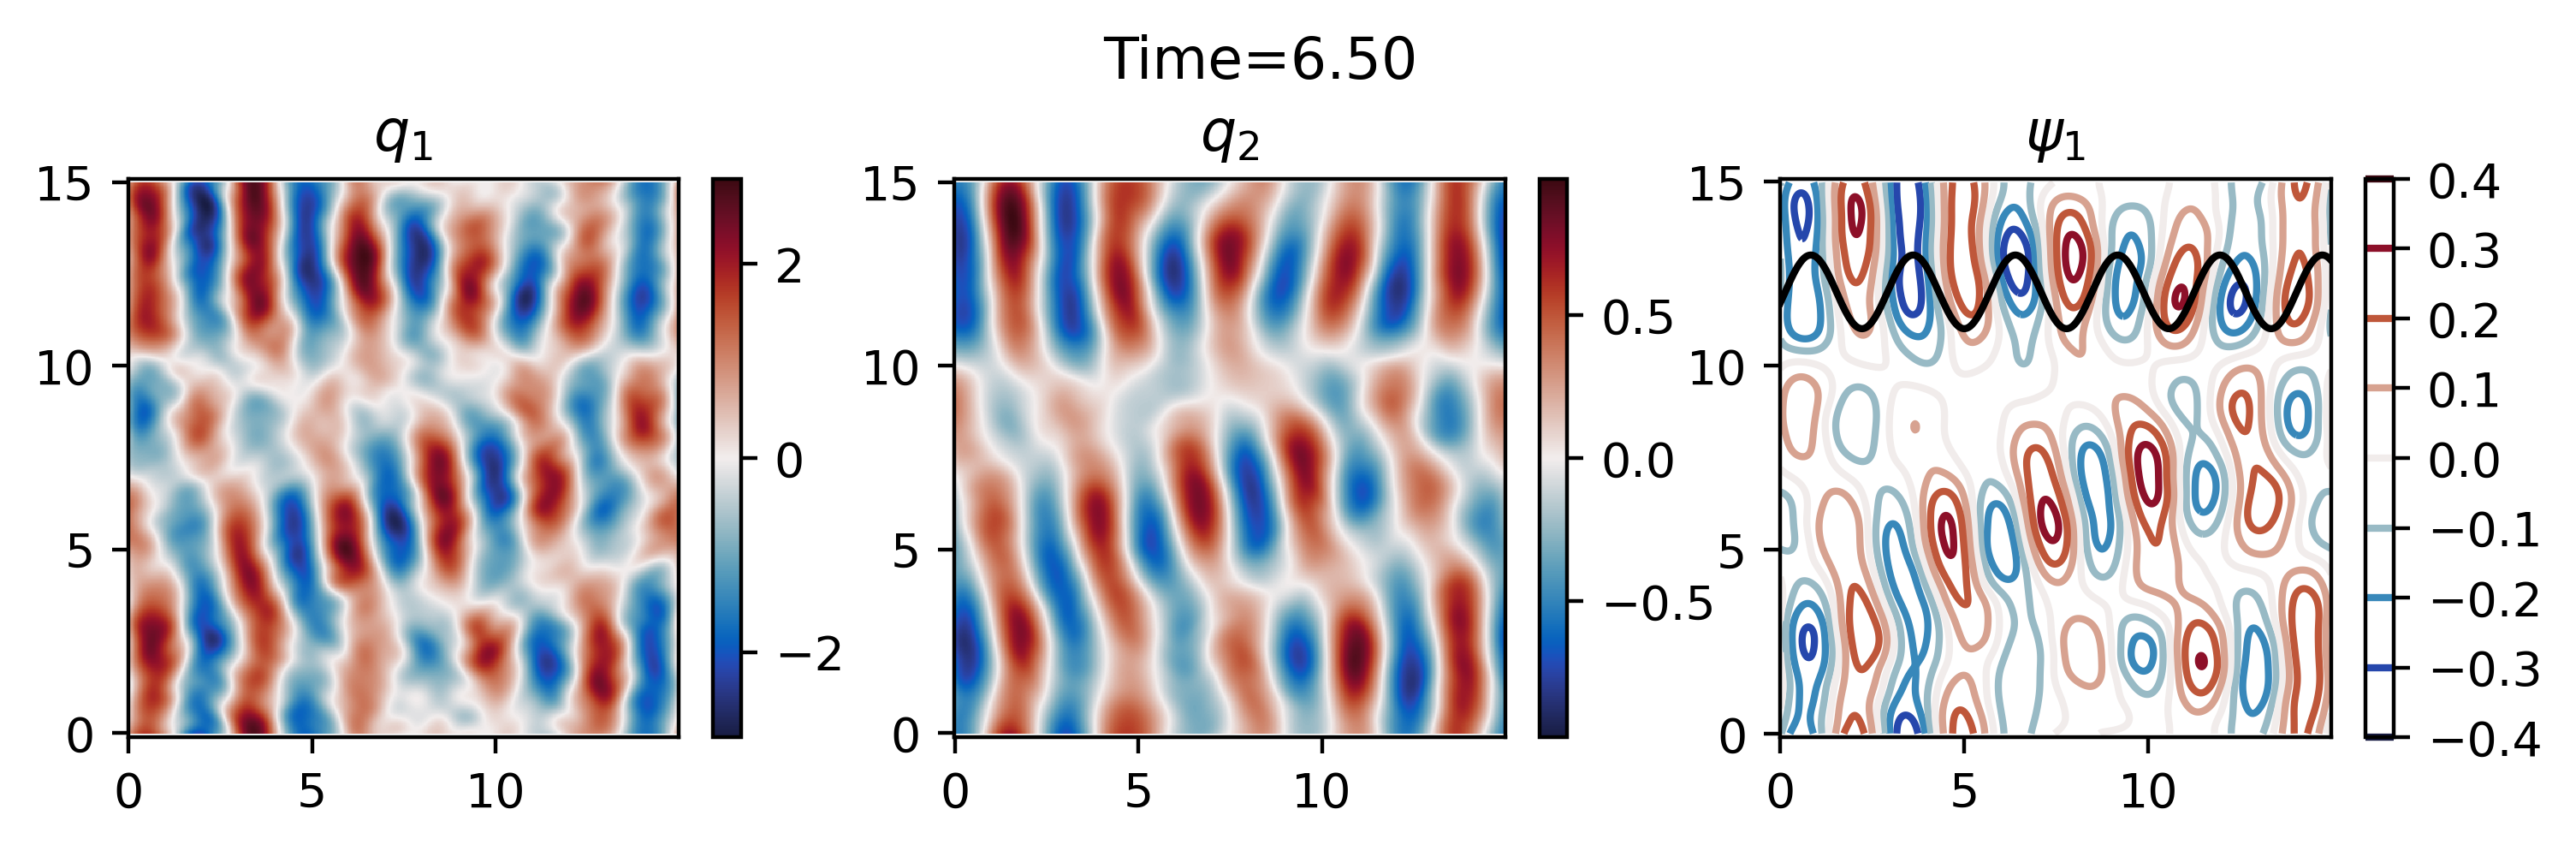
\includegraphics[width=\textwidth]{2Layjets_q1_t6d50}
    \caption{}
    \label{fig:2Layjets_q1_t6d50}
\end{figure}


\begin{figure}
    \centering
    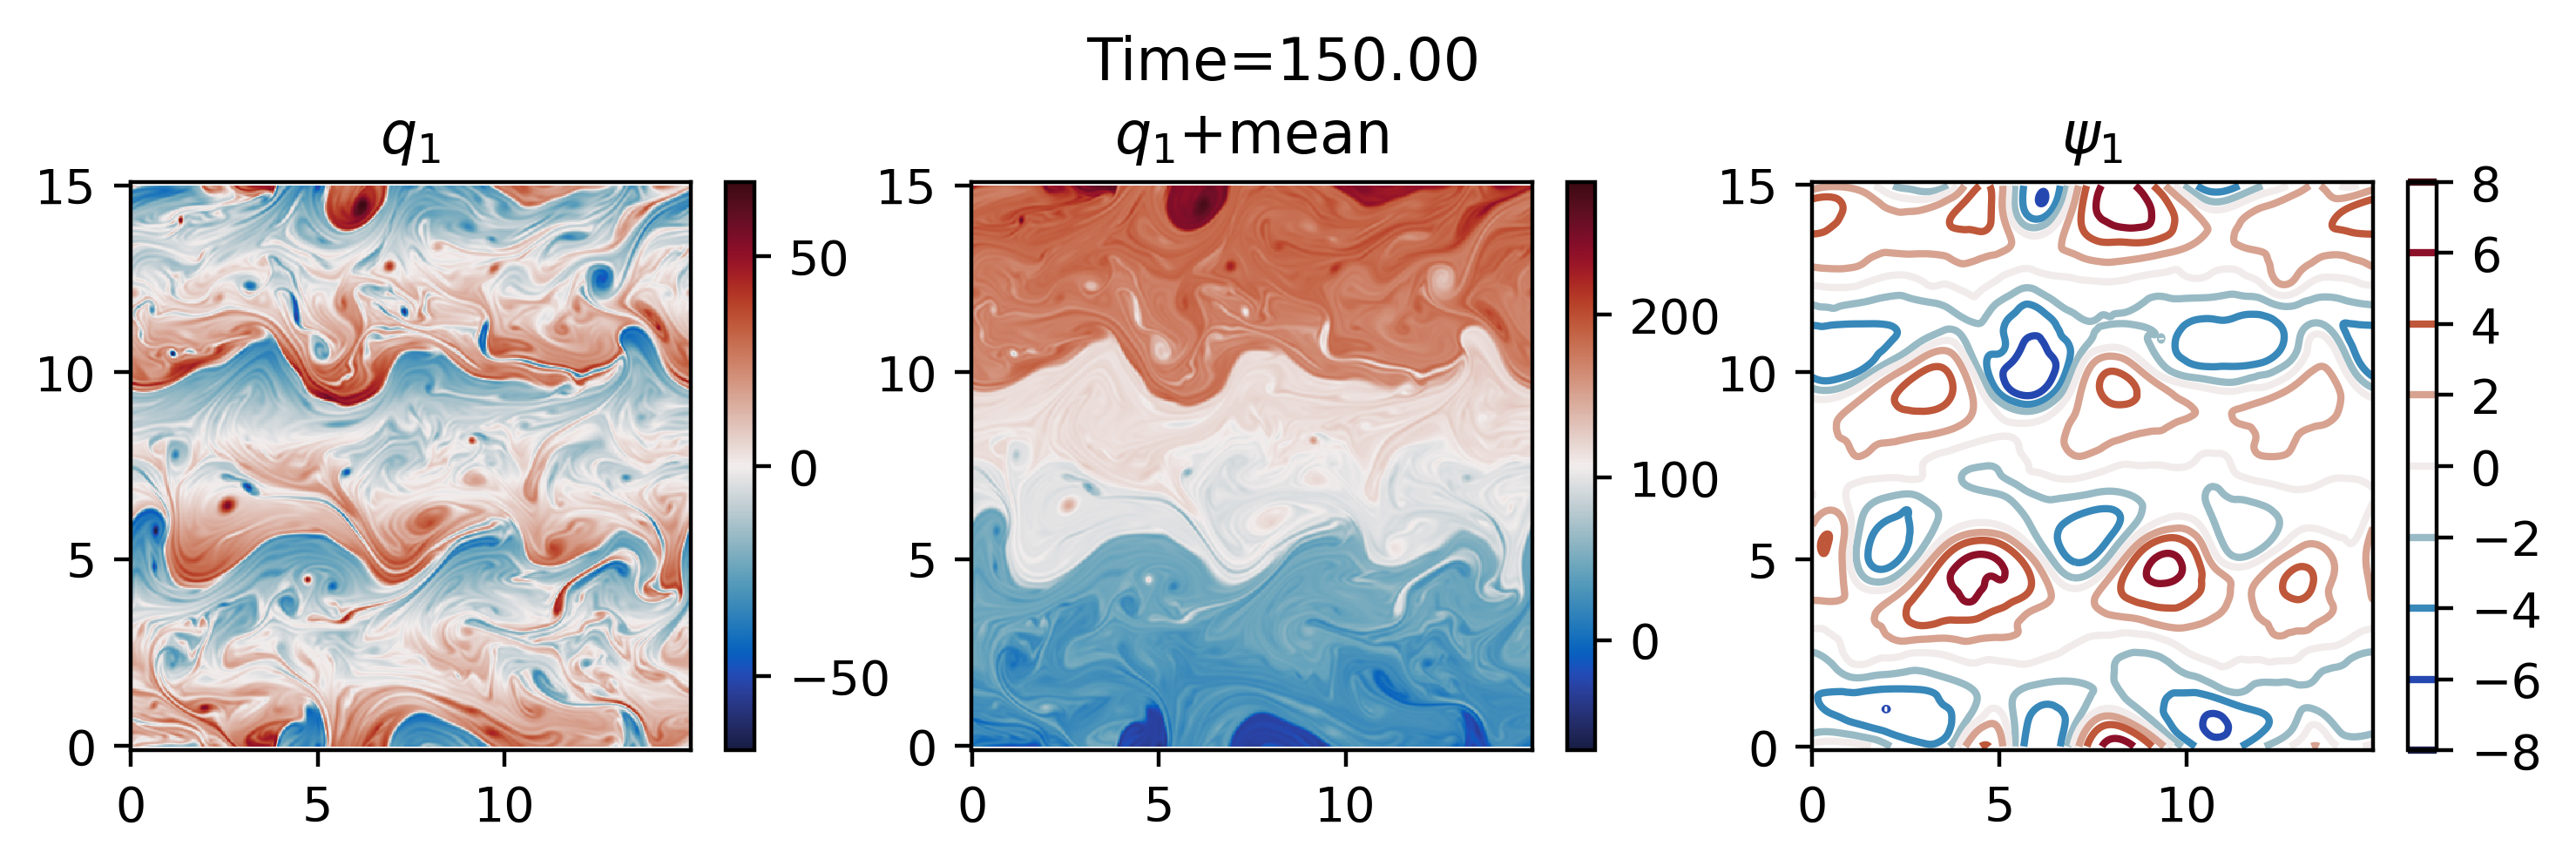
\includegraphics[width=\textwidth]{2Layjets_q1_t150d00}
    \caption{}
    \label{fig:2Layjets_q1_t150d00}
\end{figure}

\begin{figure}
    \centering
    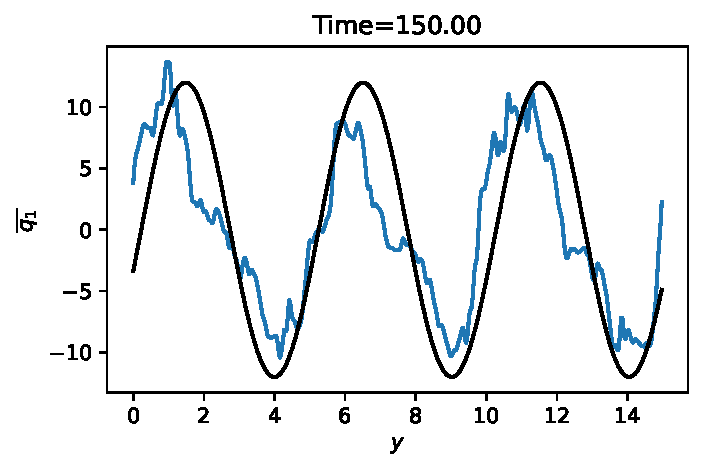
\includegraphics{2Layjets_q1zonalmean_t150d00}
    \caption{}
    \label{fig:2Layjets_q1zonalmean_t150d00}
\end{figure}

\subsection{2 layer turbulence}
We instead pick $\xi=1.5$ on a larger domain for a simulation with small $\beta$ effect. Figure \ref{fig:2Lay_qbrbc_t150d00} shows the barotropic and baroclinic PV. These are visually similar to \cite[Fig. 3]{LarichevHeld_95}. We also plot the $q_1$ enstrophy spectrum in Figure \ref{fig:2Lay_q1spec_t150d00}. The spectrum has a slope of $-1$, matching the theoretical expectation.

\begin{figure}
    \centering
    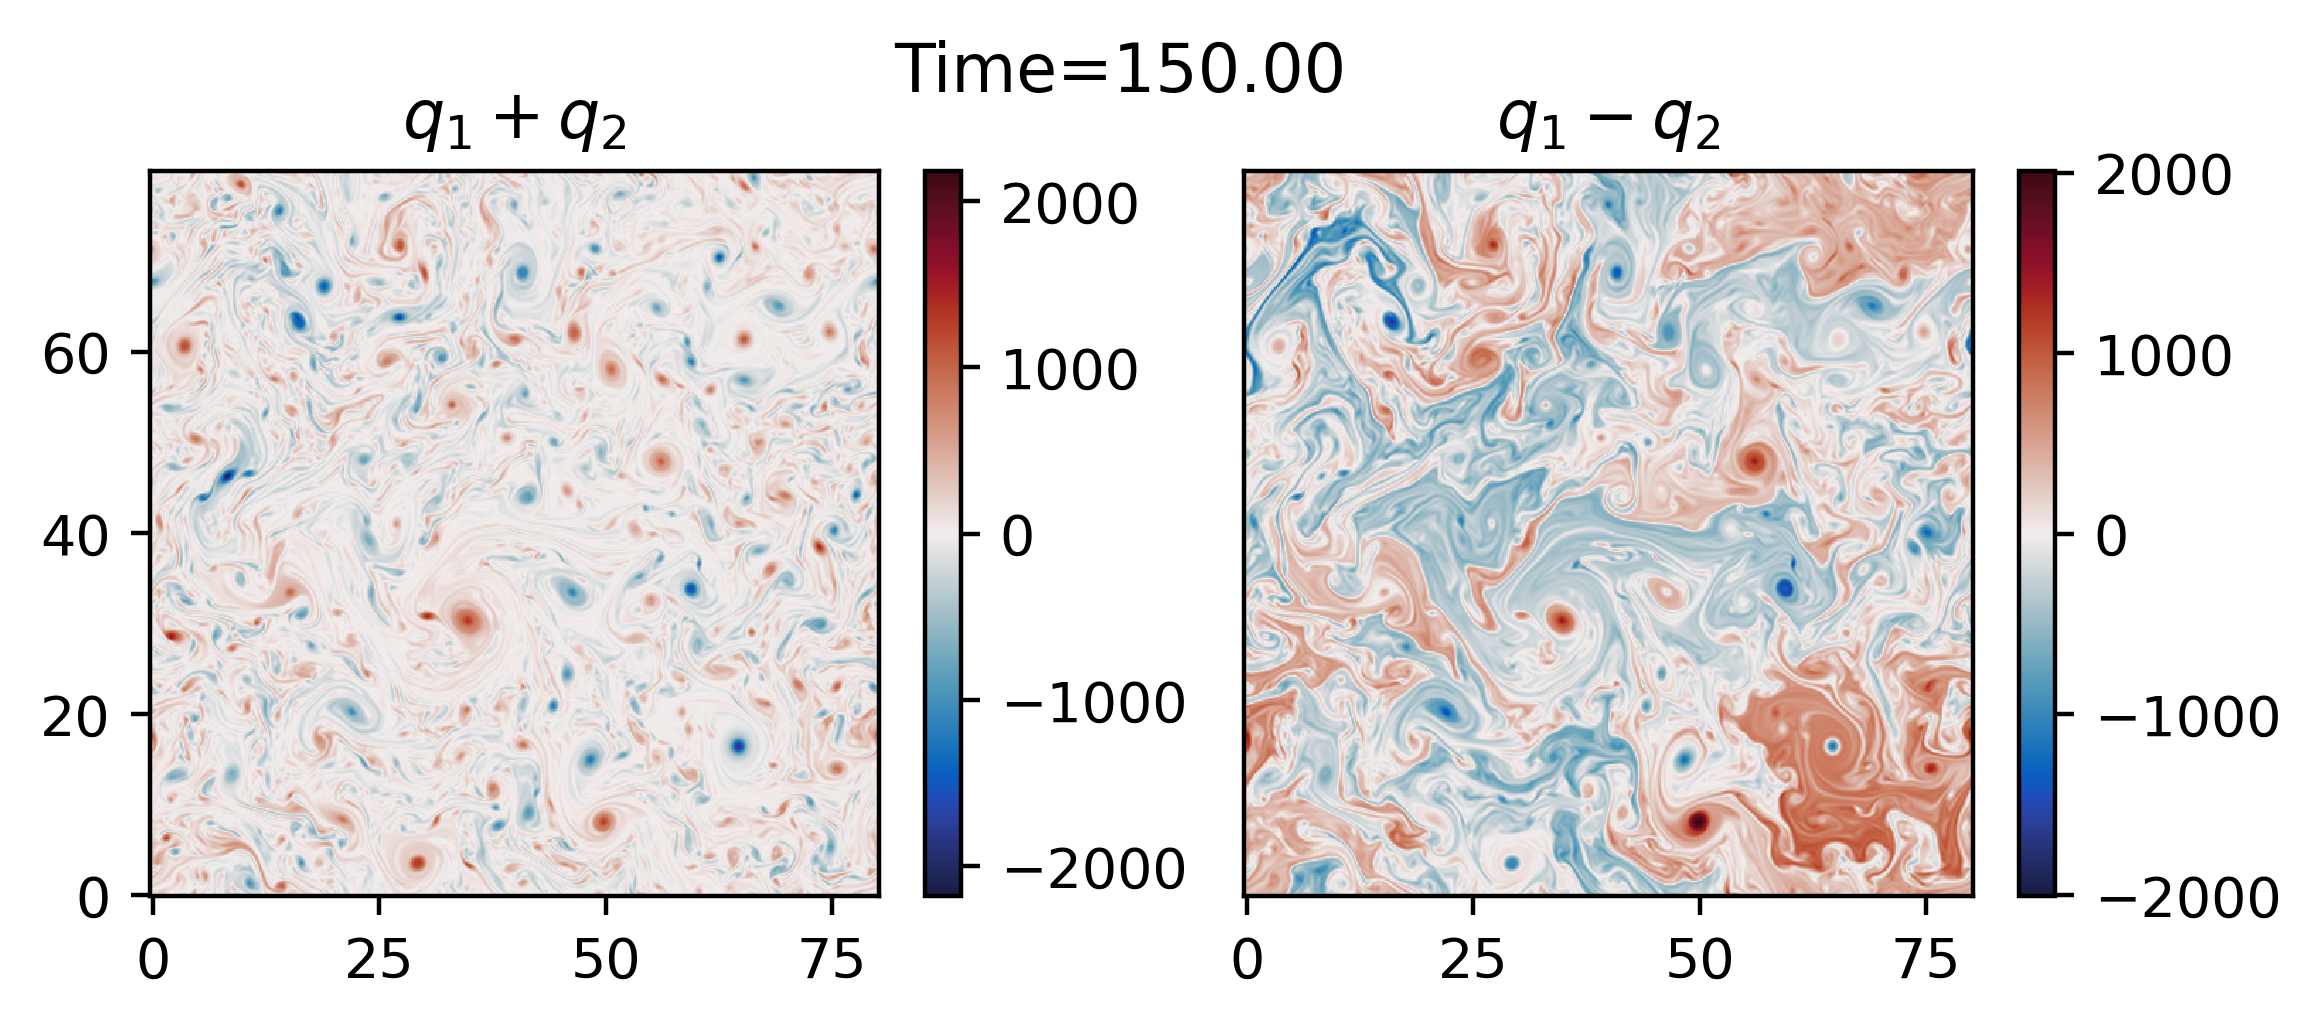
\includegraphics{2Lay_qbrbc_t150d00}
    \caption{}
    \label{fig:2Lay_qbrbc_t150d00}
\end{figure}

\begin{figure}
    \centering
    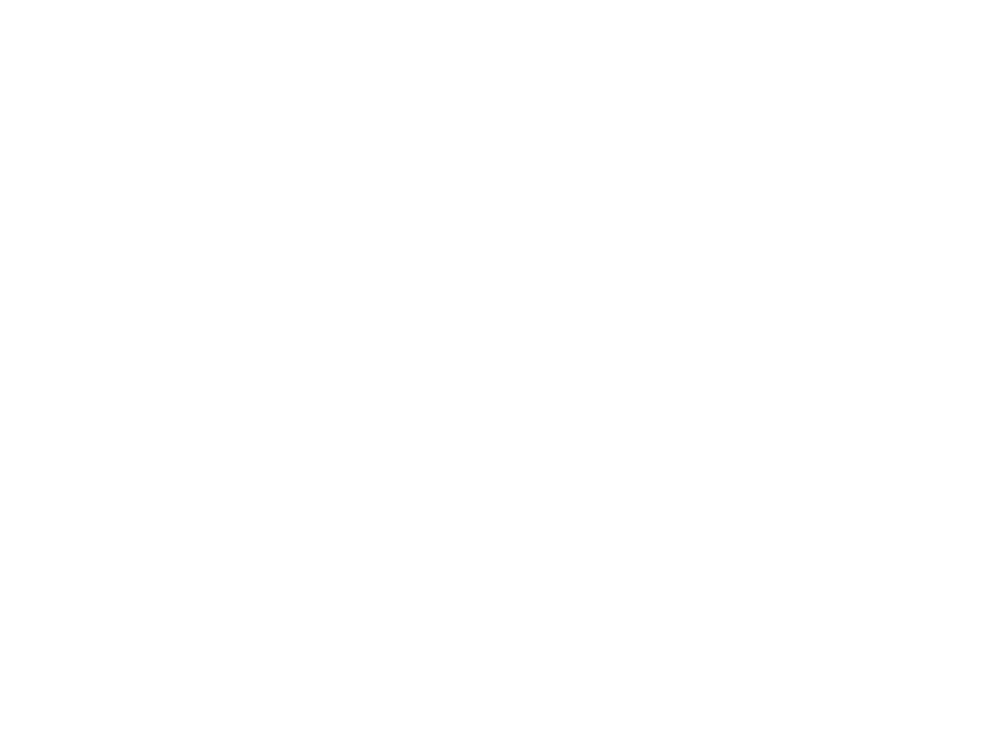
\includegraphics{2Lay_q1spec_t150d00}
    \caption{}
    \label{fig:2Lay_q1spec_t150d00}
\end{figure}